\section{Decision context and data}\label{sec:data}
The constructed system combines the supplied portfolio and simulated wind
farm \cite{brief}. Generation is fixed, demand caps sales, and neither
imports nor revenue from unused electricity enter the model.

We align five series to 2,452 UTC days (1 January 2020--17 September 2026)
and reconcile fuel totals. Repairs replace midnight snapshots with full-day
records, remove zero-volume price entries and flag estimated gaps \cite{repair}.
Daily energy is mean MW multiplied by 24~h. Prices are in 2020 pounds
using monthly consumer price indices \cite{cpi}. We size assets on 2023.

\begin{figure}[H]
  \centering
  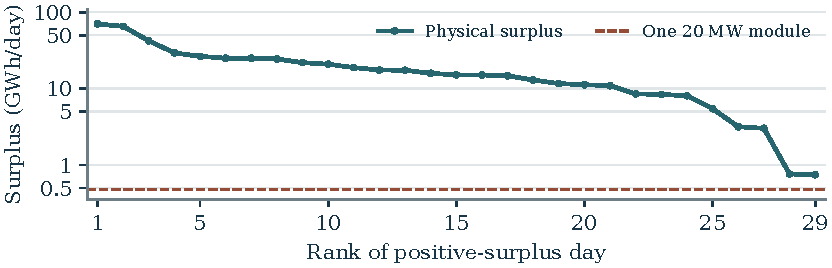
\includegraphics[width=0.94\linewidth]{figures/surplus-duration.pdf}
  \caption{Physical surplus in 2023. The 29 days with positive surplus
    total 549.94~GWh. A 20~MW module can use at most 0.48~GWh per day.}
  \label{fig:surplus}
\end{figure}

\section{Tier 1. Flexibility investment}\label{sec:tier1}
\subsection{Technology and economic assumptions}
The electrolyser capital cost uses the International Energy Agency midpoint.
Fixed operating and stack costs use UK reference estimates
\cite{dea,iea,beis}. The netback after non-power variable costs uses a
rebased policy benchmark \cite{har,cpi}. The offtake ceiling is a scenario.

\begin{table}[H]
  \centering\small
  \caption{Reference technology and valuation assumptions in 2020 pounds.}
  \label{tab:assumptions}
  \begin{tabularx}{\linewidth}{@{}lY@{}}
    \toprule
    Input & Assumption \\
    \midrule
    Battery & 1.5~MW / 3~MWh per module. 20--80\% state of charge, 90\% round-trip
      efficiency, \gbp 256,235/MWh installed, \gbp 14,862/MW-year fixed cost,
      15-year life. \\
    Electrolyser & 20~MW per module, 20--100\% online load, 55.9~kWh/kg,
      \gbp 29.21m installed and \gbp 0.517m annual fixed cost per module.
      30-year life with \gbp 9.79m stack renewals in years 11 and 22. \\
    Finance & 5\% real discount rate, \gbp 7.799/kg netback and
      10~t/day offtake ceiling. \\
    \bottomrule
  \end{tabularx}
\end{table}

\subsection{Mixed-integer formulation}\label{sec:formulation}
Let \(t\in\mathcal T\) index the days. The inputs \(G_t,D_t\) are supply and
demand in MWh, \(p_t\) is the wholesale value in \gbp/MWh, \(v\) is the hydrogen
netback in \gbp/kg and \(L\) the daily offtake limit in kg. The decision
variables \(q_t,c_t,r_t,h_t,u_t\) are direct sales, charging, discharge,
electrolyser input and unused generation in MWh. The installed battery and
electrolyser counts are \(b,n\), and \(z_t\) is the number of online
electrolyser modules. The energy requirement is \(\kappa=0.0559\)~MWh/kg.
Let \(Y\) be the number of years represented by the sample (one for a
complete calendar year), and \(a_B,a_H\) the equivalent annual costs per module.

\begin{subequations}\label{eq:tier1-model}
\begin{align}
  \max\quad & \frac{1}{Y}\sum_{t\in\mathcal T}
     \left[p_t(q_t+r_t)+v\frac{h_t}{\kappa}\right]-a_Bb-a_Hn,
       \label{eq:objective}\\
  \text{subject to}\quad
    & q_t+c_t+h_t+u_t=G_t,\qquad q_t+r_t\le D_t,
       \label{eq:balance}\\
    & c_t\le \frac{E_B}{\eta}b,\qquad r_t\le \eta E_Bb,
       \qquad \sum_{t\in\mathcal T}r_t=\eta^2\sum_{t\in\mathcal T}c_t,
       \label{eq:battery}\\
    & \underline{E}_H z_t\le h_t\le \overline{E}_H z_t,
       \qquad h_t/\kappa\le L,\qquad z_t\le n,
       \label{eq:electrolyser}\\
    & q_t,c_t,r_t,h_t,u_t\ge0,\qquad b,n,z_t\in\mathbb Z_{\ge0}.
       \label{eq:domain}
\end{align}
\end{subequations}

The day-indexed constraints hold for all \(t\in\mathcal T\).
Equation~\eqref{eq:balance} allocates generation and limits electricity sales.
The usable storage window is \(E_B=1.8\)~MWh per module and each charge or
discharge leg has efficiency \(\eta=\sqrt{0.90}\).
Equation~\eqref{eq:battery} permits one usable window of throughput per day
and balances energy over the year. In \eqref{eq:electrolyser},
\(\underline{E}_H=96\) and \(\overline{E}_H=480\)~MWh are the daily
loading limits per online module. Policy A uses the model above. Policy B
also imposes \(q_t=\min\{G_t,D_t\}\) each day.

For either technology \(j\in\{B,H\}\), the equivalent annual cost is
\begin{equation}
  a_j=F_j+\frac{i}{1-(1+i)^{-N_j}}
       \left(K_j+\sum_{k\in\mathcal R_j}\frac{C_{jk}}{(1+i)^k}\right),
  \label{eq:annual-cost}
\end{equation}
where \(i\) is the real discount rate, \(N_j\) the service life, \(F_j\)
annual fixed cost, \(K_j\) upfront investment including any commissioning
charge, and \(C_{jk}\) the renewal cost in year \(k\) of the renewal set
\(\mathcal R_j\). Each reported gain subtracts the objective value of
the zero-investment case under the same policy.

\subsection{Portfolio results and validation}\label{sec:portfolios}
FICO Xpress solves the mixed-integer program. Table~\ref{tab:portfolio}
shows the 2023 decisions. With one fixed 20~MW electrolyser, a simple
sell-first rule uses only the remaining electricity when it can meet
minimum loading. Its annual gain is \(-\)\gbp 1.07m. Economic dispatch
improves this result by \gbp 9.64m per year at the same installed capacity.

\begin{table}[H]
  \centering\small
  \caption{2023 installed capacity and equivalent annual gain relative to
    the policy-matched zero-investment case. Capacity is shown as battery /
    electrolyser in MW.}
  \label{tab:portfolio}
  \begin{tabularx}{\linewidth}{@{}Y r r r r@{}}
    \toprule
    & \multicolumn{2}{c}{A. Economic dispatch}
    & \multicolumn{2}{c}{B. Daily electricity priority} \\
    \cmidrule(lr){2-3}\cmidrule(l){4-5}
    Scenario & Capacity & {Gain (\gbp m/yr)} & Capacity & {Gain (\gbp m/yr)} \\
    \midrule
    No investment         & 0 / 0  & 0.00 & 0 / 0  & 0.00 \\
    Battery only          & 0 / 0  & 0.00 & 0 / 0  & 0.00 \\
    Electrolyser only     & 0 / 20 & 8.57 & 0 / 0  & 0.00 \\
    Joint capacity choice & 0 / 20 & 8.57 & 0 / 0  & 0.00 \\
    Fixed 20 MW module    & 0 / 20 & 8.57 & 0 / 20 & -1.07 \\
    \bottomrule
  \end{tabularx}
\end{table}

\paragraph{Battery economics.}
Even with free charging, selling a full usable discharge on every
positive-price day in 2023 yields at most \gbp 48.7k per module, below the
\gbp 96.4k annual cost. This bounds the value of adding a battery under
either policy without a minimum annual sales requirement.

\paragraph{Chronological check.}
Forcing one module in A yields \gbp 13.3k in operating value in the annual
pool. To enforce chronological operation, we impose
\begin{equation}
  s_t=s_{t-1}+\eta c_t-r_t/\eta,\qquad
  0\le s_t\le E_B b,\qquad s_0=s_{|\mathcal T|}=0,
  \label{eq:stock}
\end{equation}
where \(s_t\) is usable inventory after day \(t\). Operating value
falls to \gbp 4.3k, below even the lower fixed-cost case of
\gbp 11.1k/year. Intraday and ancillary-service revenue sit outside this
daily valuation.

\paragraph{Energy attribution.}
Of the 171.84~GWh used by the 20~MW plant, 13.92~GWh reduces unused
generation and 157.92~GWh displaces direct sales. The 13.92~GWh is 8.1\%
of the electrolyser input and 2.53\% of physical surplus.
Under a surplus-first allocation, \(C_t=\min\{h_t,\max(G_t-D_t,0)\}\).
With wind and solar generation \(R_t\), their contribution \(W_t\) to
captured surplus satisfies
\begin{equation}
  \max\{0,C_t-(G_t-R_t)\}\ \le W_t\le\ \min\{C_t,R_t\}.
  \label{eq:attribution}
\end{equation}
Summing the daily bounds gives 0--13.92~GWh. Including biomass and
run-of-river hydro leaves this interval unchanged. A narrower estimate
requires evidence on how generation is allocated.

\subsection{Contract terms and service requirements}\label{sec:contracts}
Figure~\ref{fig:contract} varies the netback and daily acceptance cap
together. At 10~t/day, the 20~MW module breaks even at \gbp 4.61/kg in A
and \gbp 12.08/kg in B. In A, installing 40~MW under the same cap increases
hydrogen sales but lowers the gain to \gbp 7.47m/year. At 50~t/day, A
chooses 120~MW and gains \gbp 49.09m/year on \gbp 175.25m of initial
capital, conditional on the larger contract.

\begin{figure}[H]
  \centering
  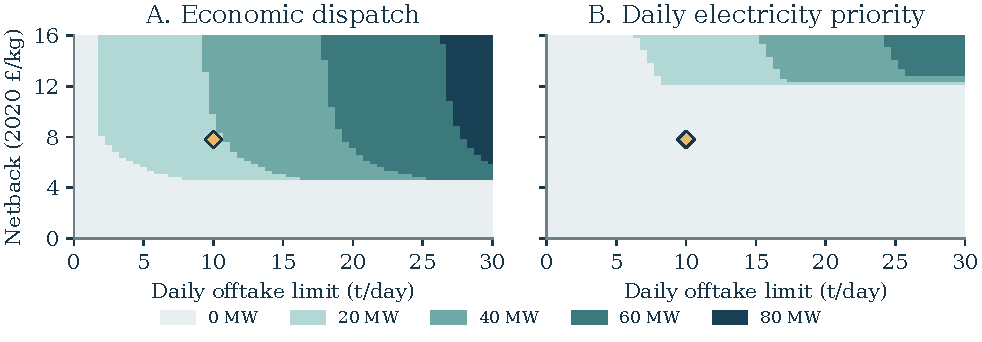
\includegraphics[width=\linewidth]{figures/contract-trigger.pdf}
  \caption{Optimal electrolyser capacity for alternative 2023 contracts.
    Diamonds mark the reference terms. The colours show installed capacity
    in multiples of 20~MW.}
  \label{fig:contract}
\end{figure}

Table~\ref{tab:sales-floor} sets annual sales floors relative to the
215.1~TWh sold in the A zero-investment case. An annual floor permits the
operator to choose the days on which to preserve sales. Policy B gives
electricity sales priority every day.

\begin{table}[H]
  \centering\small
  \caption{Annual electricity sales retained under A. The first row is
    the unrestricted outcome. The remaining rows impose a minimum.}
  \label{tab:sales-floor}
  \begin{tabularx}{\linewidth}{@{}Y r r
    r r@{}}
    \toprule
    Scenario & {Sales retained (\%)} & {Sales given up (GWh)}
      & {\hydrogen{} (MW)} & {Gain (\gbp m/yr)} \\
    \midrule
    Unrestricted          & 99.9266 & 157.92 & 20 & 8.57 \\
    Restore half the loss & 99.9633 &  78.96 & 20 & 5.19 \\
    Tight sales floor     & 99.9900 &  21.51 & 20 & 1.04 \\
    Preserve all sales   & 100.0000 &   0.00 &  0 & 0.00 \\
    \bottomrule
  \end{tabularx}
\end{table}

\paragraph{Result checks.}
We reconciled energy, equipment limits and revenues in 42 optimal and
two rule-based schedules. Physical residuals are below 0.001~MWh.
Xpress confirms eight trigger points, the capacity checks and the sales
floors. A separate implementation agrees on 18 matched cases.

\begin{samepage}
\subsection{Robustness and returns}
We hold the electrolyser at 20~MW and reoptimise dispatch on each realised
calendar year. The site-only check gives background generation priority
on demand and restricts the device to wind-farm output.
Table~\ref{tab:replay} reports gains against the corresponding
zero-investment case. Under B, the break-even netback falls to
\gbp 3.13/kg in 2025 as surplus increases, but lowering both netback
and offtake reverses the result. In 2023, A still gains \gbp 7.29m/year
with 25\% higher installation cost and an 8\% real discount rate.
Reoptimising on the 280 strict-quality days retains the original capacities.
\end{samepage}

\begin{table}[H]
  \centering\small
  \caption{Fixed 20~MW replays. Gains are in \gbp m/year, 2020 prices.}
  \label{tab:replay}
  \begin{tabularx}{\linewidth}{@{}Y r r@{}}
    \toprule
    Period and assumptions & {A. Economic dispatch} & {B. Daily electricity priority} \\
    \midrule
    2022 & 8.91 &  7.31 \\
    2023 & 8.57 & -1.07 \\
    2024 & 11.95 & -1.00 \\
    2025 & 13.17 &  4.48 \\
    2025, \gbp 4/kg and 5~t/day & -0.24 & -0.77 \\
    2023, wind-site boundary   &  8.17 & -1.07 \\
    \bottomrule
  \end{tabularx}
\end{table}

\begin{table}[H]
  \centering\small
  \caption{Annual value bridge for A, 2023, 20~MW.}
  \label{tab:value}
  \begin{tabularx}{\linewidth}{@{}Y r@{}}
    \toprule
    Component & {Value (\gbp m/year)} \\
    \midrule
    Hydrogen netback receipts                    & 23.97 \\
    Forgone direct electricity receipts          & -12.39 \\
    Fixed operating cost                         & -0.52 \\
    Equivalent cost of capital and stack renewals & -2.49 \\
    \midrule
    Equivalent annual gain                      & 8.57 \\
    \bottomrule
  \end{tabularx}
\end{table}

The \gbp 29.21m upfront cost and \gbp 11.06m annual operating cash flow
give a 2.64-year simple payback and a 2.90-year discounted payback.
Repeating the 2023 operating cash flow for 30 years with renewals in
years 11 and 22 and zero terminal value gives a net present value of
\gbp 131.78m. The annual value bridge is given in Table~\ref{tab:value}.
